\section{Implementation des Moduls zur Verhaltensklassifizierung} \label{sec:umse ModulKonzept}
Für das Modul sind viele der bereits vorgestellten Umsetzungen übernehmbar. Die Feature-Extraktion lässt sich genau wie in \autoref{secc:Umsetz Featextr} beschrieben, in das Modul integrieren. Lediglich kleine Anpassungen werden vorgenommen. Z.B. anstatt, dass die Feature-Extraktion die Dateipfade übergeben bekommen, wie im Codeauszug \ref{lst:FE IterInterv} gezeigt, bekommt sie im Modul die Daten direkt übergeben. Auch die Formatierung und das Assoziationsmodul sind hier implementiert. Die Skalierung wird so integriert, wie in \autoref{sec:umsetz FeatSelec}. Während des Modellaufbaus wird der Skalierer trainiert und gespeichert und kann anschließend in das Modul eingebaut werden. Die polynomiale SCM wird trainiert und getestet, wie in \autoref{sec:umsetz FeatSelec} gezeigt wird und ist anschließend in das Modul zu laden. Bezogen auf das Konzept in \autoref{sec:Meth Sim} ist somit die Implementation von allen Komponenten erläutert, bis auf die des Pufferspeichers und die des Ringpufferspeichers. Aus diesem Grund werden die bereits beschriebenen Komponenten in diesem Kapitel nicht mehr im Detail erläutert.\par

Um das Modul zu testen, ist eine Simulation geplant. Dazu wird eine Simulation des Rohdatenstroms benötigt. Das Kapitel wird vor dem Hintergrund der Simulation strukturiert. Zunächst wird die Umsetzung der Simulation des Rohdatenstroms beschrieben und anschließend folgt Darstellung der Modul-Implementation.

\subsection{Umsetzung der Simulation des Rohdatenstroms}

\begin{figure}[p]
    \centering
    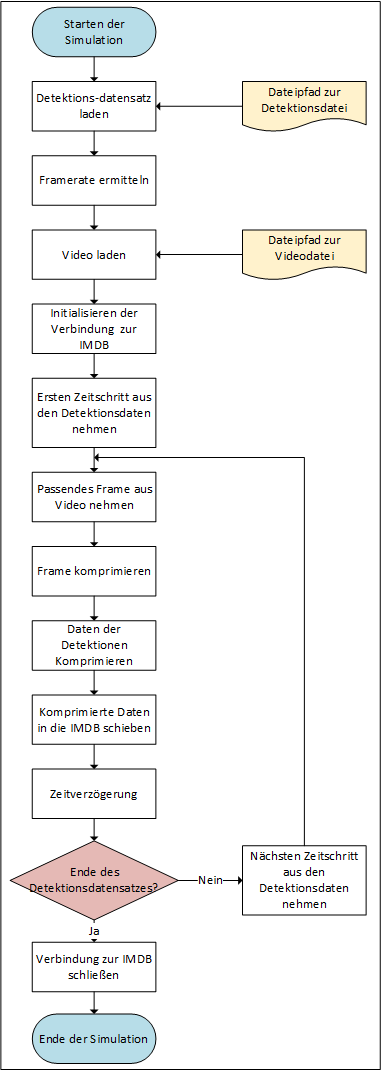
\includegraphics[height=0.9\textheight]{img/Grafiken/Flussdiagramm Simulation Rohdatenstrom.png}
    \caption{Flussdiagramm des Programmablaufs der Simulation des Rohdatenstroms.}
    \label{fig:FlussDia SimStream}
\end{figure}

Die Simulation des Rohdatenstroms lässt sich in drei Blöcke zerlegen. Einer Konfiguration, in welcher die notwendigen Vorbereitungen getroffen werden, dem Anknüpfen an den Pufferspeicher und dem Simulieren des Datenstroms. Im Flussdiagramm aus \autoref{fig:FlussDia SimStream} sind diese drei Blöcke zusammen mit den Programmschritten zu sehen, welche in ihnen stattfinden. \par


Das Programm beginnt mit der Konfiguration der Dateipfade. Diese werden explizit in den Code geschrieben. Um die Framerate zu simulieren, wird die mittlere Zeitschrittweite zwischen zwei Frames ermittelt. Dazu wird der Detektionsdatensatz mit \textit{pandas} geladen. Über den Zeitstempel in Unixzeit und internen Methoden von \textit{pandas} ist die mittlere Zeitschrittweite in Sekunden zu berechnen. Das ist im Codeauszug \ref{lst:deltaTframrate} zu sehen.

\begin{pythoncode}{Ermittlung der mittleren Zeitschrittweite der Einträge in einem Detektionsdatensatz.}{lst:deltaTframrate}
#Mittlere Zeitschrittweite der Frames in Sekunden 
df = pd.read_csv(csv_file_path)
dTime_frame = df['timestamp_server'].diff().mean()/1000
\end{pythoncode}

Der Pufferspeicher ist als In-Memory Datenbank realisiert. Die Software \textit{Redis} implementiert IMDBs. Es existiert eine gleichnamige Bibliothek, mit welcher der Zugriff über Python-Code möglich ist. Die Datenbank wird lokal auf dem Rechner realisiert. Im Codeauszug \ref{lst:redisConfig} ist die Einrichtung und der Aufbau der Verbindung zur IMDB zu sehen.

\begin{pythoncode}{Verbidnungsaufbau zur IMDB.}{lst:redisConfig}
import redis
#Redis-Verbindung einrichten
redis_client = redis.StrictRedis(
                    host='127.0.0.1',
                    port=6379,
                    decode_responses=True)
\end{pythoncode}

Um den Rohdatenstrom zu realisieren, sind die Dateien einzulesen. Das Video wird über \textit{OpenCV} geladen. Für die Detektionsdaten wird diesmal die Bibliothek \textit{csv} verwendet. Während zuvor oft \textit{pandas} angewendet wurde, welche auf Datenanalyse ausgelegt ist, ist \textit{csv} auf das Lesen und Schreiben von csv-Dateien spezialisiert. Im Codeauszug \ref{lst:loadDetsNVid} werden die Detektionsdatei und die Videodatei geöffnet. Aus dem Detektionsdatensatz wird die erste Zeile gelesen. Dabei handelt es sich um die Kopfzeile mit den Spaltennamen. Diese werden für später gespeichert. 

\begin{pythoncode}{Laden der Detektionsdatei und des Videos.}{lst:loadDetsNVid}
import csv
#csv-Datei zum Lesen öffnen 
with open(csv_file_path, 'r', newline='', encoding='utf-8') as csv_file:
    csv_reader = csv.reader(csv_file)

    #Kopfzeile speichern
    headers = next(csv_reader)
    headers.append("frame")

    #Video Laden
    vidCap = cv2.VideoCapture(video_path)
\end{pythoncode}

Die Detektionsdatei wird Eintrag für Eintrag durchiteriert. Das Video wird auf das Startframe gesetzt. Das erfolgt über die Frame-ID im Detektionsdatensatz. Anschließend wird bei jeder Iteration das nächste Frame geladen. Das ist im Codeauszug \ref{lst:LoopVidDets} zu sehen. Die if-Abfrage dient dazu, dass das Startframe nur zu Beginn gesetzt wird. Für die prinzipielle Funktion wäre ein wiederholter Aufruf von \textit{vidCap.set} nicht schädlich, jedoch führe dies zu vermeidbarem Overhead. Die Zeitabfrage wird für die Ermittlung der Verzögerung benötigt, um die Framerate zu simulieren. Der Befehl \textit{time.time()} gibt die Sekundenanzahl seit Programmstart zurück.


\begin{pythoncode}{Iteration durch die Rohdaten für einen schrittweisen Datenstrom.}{lst:LoopVidDets}
#Durchlaufen der CSV-Datei Zeile für Zeile
for i, row in enumerate(csv_reader):

    #Zum Messen der Prozessdauer
    start_time = time.time()
    
    #Cursor bei Beginn auf das Startframe setzen
    if startframe_set is False:
        vidCap.set(1, int(row[0])-1)
        startframe_set = True

    #Frame Laden                          
    _, frame = vidCap.read()
\end{pythoncode}

Bilder können viel Speicherplatz benötigen. Da der Datenfluss durch eine Speicherung im Arbeitsspeicher läuft, ist die Datengröße zu minimieren. Das reduziert die Anforderungen an den Rechner, auf welchem das Modul laufen soll. Im Codeauszug \ref{lst:kompFrame} ist deshalb zu sehen, wie das Frame komprimiert wird. Dazu wird die \textit{PIL} Bibliothek verwendet, eine Bibliothek für die Bildverarbeitung. Das Frame wird als Matrix eingelesen. Jedes Matrixelement ist ein Pixel, welcher aus einem Array für die RGB-Werte  besteht. Diese Matrix wird in ein \textit{Image}-Objekt der \textit{PIL} Bibliothek umgewandelt. Dadurch kann es PNG-Codiert werden. Über die Bibliothek \textit{io} wird die Byte-Folge des PNG-Bildes ermittelt und mit der Bibliothek \textit{Base64} wird die Byte-Folge als utf-8 Codierung interpretiert. Diese Codierung wird dem Eintrag der Detektionsdaten angehangen. Dadurch wird eine geschlossene Übertragung, der Daten zu einem Zeitschritt in die IMDB erzielt.

\begin{pythoncode}{Komprimierung und Codierung des Frames.}{lst:kompFrame}
from PIL import Image
#Konvertieren des Frames in ein PIL Image-Objekt
image = Image.fromarray(frame.astype('uint8'), 'RGB')

import io
#Komprimieren und Speichern des Frames als PNG
img_byte_arr = io.BytesIO()
image.save(img_byte_arr, format='PNG')

#Konvertieren des PNG in Bytes
img_bytes = img_byte_arr.getvalue()

import base64
#Frame utf-8 Codieren
#Wird für die Speicherung im JSON-Format benötigt
img_base64 = base64.b64encode(img_bytes).decode('utf-8')

#Frame den Daten beifügen
row.append(img_base64)
\end{pythoncode}

Der komplette Dateneintrag des Zeitschritts wird zusätzlich codiert und komprimiert. Im Codeauszug \ref{lst:KompCodePuff} ist zu sehen, dass die Daten als JSON-String verpackt werden. Dabei werden die Daten im Eintrag der entsprechenden Zeilenüberschrift aus der Kopfzeile zugeordnet. Das dient der vereinfachten Handhabung und Interpretation im Modul. Der String wird utf-8 codiert, komprimiert und ins Hexadezimal-Format gebracht. Der Hexadezimal-String wird in die IMDB geschoben. In der Datenbank wird ein Listen-Objekt mit dem Namen \textit{fifo\_mem} initialisiert. Diese Liste ermöglicht die FIFO-Arbeitsweise des Pufferspeichers.

\begin{pythoncode}{Komprimierung und Codierung des gesamten Zeitschritts und Schieben in den Puffer.}{lst:KompCodePuff}
import json
#Daten als JSON-String verpacken
json_string = json.dumps({header: value for header, value in zip(headers, row)}).encode('utf-8')

import zlib
#Komprimierung des JSON-String 
comp_data = zlib.compress(json_string).hex()

#Schiebe die Daten in die IMDB
redis_client.lpush("fifo_mem", comp_data)
\end{pythoncode}

Am Ende der Iteration ist eine Verzögerung eingebaut. Diese wird berechnet aus der Differenz der mittleren Zeitschrittweite \textit{dTime\_frame} und der Verarbeitungszeit. Die Verarbeitungszeit wird über die Variable \textit{start\_time} aus dem Codeauszug \ref{lst:LoopVidDets} berechnet. Die Einstellung der Verzögerung ist im Codeauszug \ref{lst:delay FramRate} zu sehen.

\begin{pythoncode}{Verzögerung der nächsten Iteration zur  Simulation der Framerate.}{lst:delay FramRate}
#Dauer des Durchlaufs bestimmen 
end_time = time.time()
execution_time = end_time - start_time 

#Verzögerung berechnen, zur Simulation der Framrate
sleep_time = dTime_frame - execution_time 
if sleep_time > 0:
    time.sleep(sleep_time)  # Warten, falls nötig
\end{pythoncode}


\subsection{Umsetzung des Moduls}

\begin{figure}[p]
    \centering
    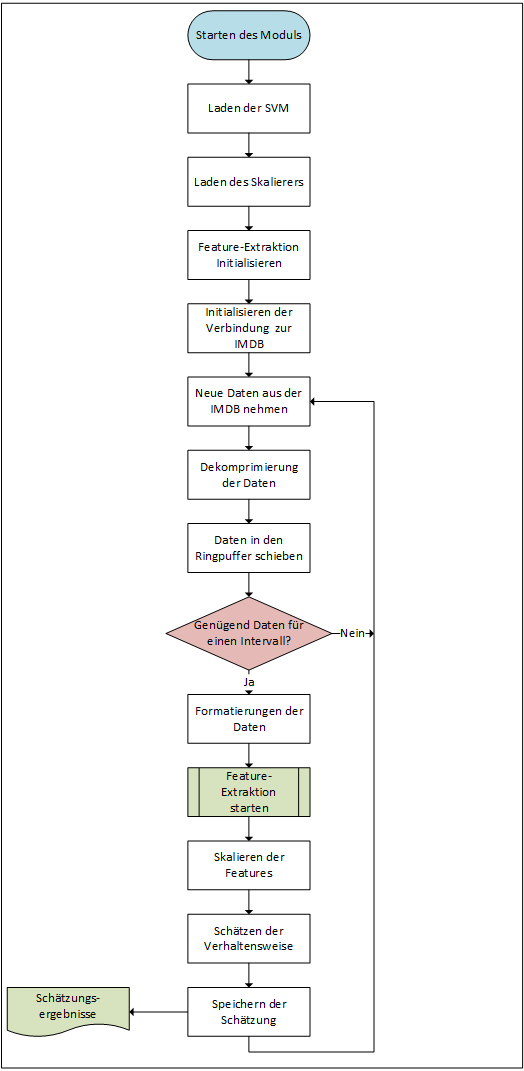
\includegraphics[height=0.9\textheight]{img/Grafiken/Flussdiagramm Modul.png}
    \caption{Flussdiagramm des Programmablaufs der Modul-Implementaion.}
    \label{fig:FlussDia Modul}
\end{figure}

Der Ablauf des Programms des Moduls lässt sich unterteilen in eine Initalisierungsblock, den Verbindungsaufbau zum Pufferspeicher und einer Routine, bestehend aus der Erhebung der Daten im Pufferspeicher in den Ringpufferspeicher und der Verarbeitung eines Intervalls. Das Flussdiagramm \autoref{fig:FlussDia Modul} zeigt den Programmablauf der Implementation des Moduls. \par

In Bezug auf das Konzept in \autoref{sec:Meth FinalKonzept} sind im Flussdiagramm die Verbindungen der Speicher zu erkennen. Die Formatierung, die Assoziation und die Feature-Extraktion sind in dem Programmschritt der Feature-Extraktion implementiert, wie in \autoref{secc:Umsetz Featextr} beschrieben. Die Skalierung der Features sowie die Schätzung der Verhaltensweise durch das Modul sind klar im Flussdiagramm zu erkennen. \par

Für die Modulimplementierung müssen einige Elemente aus dem Modellaufbau extrahiert werden, um sie anschließend einbinden zu können. Das beinhaltet die trainierte SVM, den Skalierer und die Intervalle für die Gruppierung der Quantil-Features. Das ist notwendig, damit nach der Implementation des Moduls die Trainingsdaten vollständig verworfen werden können. Im Codeauszug \ref{lst:saveElems} sind die wichtigsten Programmzeilen des Modellaufbaus zu sehen, um die notwendigen Informationen zu extrahieren.\par

Über die Bibliothek \textit{joblib} und dem Befehl \textit{dump} können beliebige Python-Objekte als Datei gespeichert werden. So werden der Skalierer und das Modell gesichert. Im Modul können die Dateien ebenfalls mit \textit{joblib} geladen werden, wie im Codeauszug \ref{lst:loadModSkal}. Die Intervalle der Quantil-Features werden in einer json-Datei gespeichert. Json eignet sich, um Daten strukturiert zwischen Programmen auszutauschen. Die json-Datei wird in der Feature-Extraktion gelesen über die Methode \textit{load\_bins\_from\_json} und \textit{pandas} nutzt die Intervalle für die Zuordnung neuer Feature-Werte.

\begin{pythoncode}{Extraktion der Elemente aus dem Modellaufbau zur Integration in das Modul.}{lst:saveElems}
#Speichern der Skalierung 
joblib.dump(scaler, 'MinMaxScaler.joblib')

#Speichern des trainierten Models
joblib.dump(svm_classifier, 'Trained_SVC_Classifier.joblib')


#Quantil-Einteilung aus json-Datei laden
bin_intervals = load_bins_from_json()

#Iterieren durch die zu gruppierenden Spalten
#Neue Features der entsprechenden Gruppe zuordnen 
quantil_cols[f'quantil_{column}'] = pd.cut(features[column], 
                                       bins=bin_intervals[f'quantil_{column}'])
\end{pythoncode}                                       

Mit dem Befehl \textit{load} lassen sich Modell und Skalierer einfach laden und in das Modul integrieren. 

\begin{pythoncode}{Laden der Elemente aus dem Modellaufbau in das Modul.}{lst:loadModSkal}
#Laden des Modells und des Skalierers
svm_classifier = joblib.load('Trained_SVC_Classifier.joblib') 
minmax_scaler = joblib.load('MinMaxScaler.joblib')
\end{pythoncode}

Im Codeauszug \ref{lst:initsModul} ist die Initialisierung der Feature-Extraktion zu sehen und die Initialisierung der Anknüpfung an die IMDB für den Zugriff auf den Pufferspeicher. 

\begin{pythoncode}{Initalisierungen für das Modul.}{lst:initsModul}
#Feature Extraktor initialisieren
feat_extr = FeatureExtractor()

#redis verbindung initialisieren
redis_client = init_redis_connection()
\end{pythoncode}

Nach den Initialisierungen wird die Routine des Moduls gestartet. Dafür wird eine Endlosschleife verwendet. Das zeigt der Codeauszug \ref{lst:puffToRing}. Die Funktion \textit{get\_new\_entries} fragt den Pufferspeicher ab, ob neue Daten vorhanden sind. Ist das der Fall, werden diese aus dem Puffer geladen. Der Eintrag wird dabei aus dem Puffer entfernt. Das Laden erfolgt nach dem FIFO Prinzip. Die Funktion \textit{update\_data\_list} implementiert das Ringpuffer-Prinzip. Die Liste \textit{data\_list} stellt den Ringpufferspeicher dar. In der Funktion wird dafür gesorgt, dass sich in der Liste nur die aktuellsten 40 Sekunden befinden.  \par

In der Funktion \textit{get\_new\_entries} ist ebenfalls die Decodierung und die Dekomprimierung der Daten implementiert. Die Abfolge der Schritte ist genau entgegengesetzt zu Codierung und Komprimierung und erfolgt mit den entsprechenden Umkehrbefehlen.

\begin{pythoncode}{Erhebung der Pufferdaten in den Ringpufferspeicher.}{lst:puffToRing}
data_list = []
while True:

    #Daten aus dem Puffer in den Ringpuffer schieben
    new_entries = get_new_entries(redis_client)

    #Implementiert Ringpuffer-Mechanik
    #Neue Daten überschreiben die Ältesten
    data_list = update_data_list(data_list, new_entries)
\end{pythoncode}

Ist der Ringpuffer voll, ist ein vollständiges Intervall für die Auswertung bereit. Eine if-Abfrage kontrolliert, ob genügend Daten vorhanden sind. Das wird im Codeauszug \ref{lst:startAuswert} abgebildet. Vor der Übergabe an die Feature-Extraktion werden die Detektionsdaten zu einem Dataframe formatiert. Die Videoframes werden als Liste verpackt. 

\begin{pythoncode}{Beginn der Auswertung eines Intervalls.}{lst:startAuswert}
#Kontrolle, ob ein volles Intervall im Ringpuffer liegt
if check_if_enough_data(data_list):

    #Intervalldaten als DataFrame formatieren 
    data = pd.DataFrame(data_list)

    #Frames und Detektionsdaten trennen 
    frames = data['frame'].to_list()
    dets = data.drop('frame', axis=1)
\end{pythoncode}

Im Codeauszug \ref{lst:startExtr} ist die Übergabe an die Feature-Extraktion zu sehen. Dies funktioniert wie in \autoref{secc:Umsetz Featextr} dargestellt. Die Klasse \textit{detectionDataHandler} ist eine Hilfsklasse, welche die Informationen aus den Detektionen strukturierter zugänglich macht. 

\begin{pythoncode}{Übergabe der Daten an die Feature-Extraktion.}{lst:startExtr}
#Extrahieren der Daten zum Intervall 
detData_handler = detectionDataHandler(data)

#Informationen an die Feature-Extraktion weitergeben
features = feat_extr.get_features(detData_handler.data, 
                                frames, 
                                detData_handler.startTime, 
                                detData_handler.endTime, 
                                detData_handler.kameraID)
\end{pythoncode}

Nach der Feature-Extraktion werden diese vom Skalierer richtig skaliert und anschließend dem Modell übergeben. Dieses schätzt auf Basis der Daten die Verhaltensweise. Für eine Auswertung wird das Schätzungsergebnis sowie Start- und Endzeitpunkt des Intervalls in einer csv-Datei gespeichert. Das zeigt der Codeauszug \ref{lst:modelResSave}.

\begin{pythoncode}{Skalieren der Features und Auswertung der Verhaltensweise.}{lst:modelResSave}
#Features Skalieren
x_scaled = minmax_scaler.transform(features) 

#gebe die Features in den Klassifizierer
label = svm_classifier.predict(x_scaled)

#Speichern des Klassifizierungsergebnis
prediction_to_csv(label, 
                  features['Startzeit'].iloc[0], 
                  features['Endzeit'].iloc[0])
\end{pythoncode}


                